\documentclass[12pt]{article}

% Packages
\usepackage[utf8]{inputenc}
\usepackage{amsmath}
\usepackage{amsfonts}
\usepackage{amssymb}
\usepackage{graphicx}
\usepackage{hyperref}
\usepackage{tikz}
\usepackage{fancyvrb}
\usepackage{multicol}
\usepackage{array}
\usepackage{amsmath}
\usepackage{tabularx}
\usepackage{tcolorbox}
\usepackage{float}

\usetikzlibrary{arrows.meta}
\hypersetup{
    colorlinks=true,
    linkcolor=black,
    citecolor=black,
}
\newenvironment{code}{\fontfamily{zi4}\selectfont}{\par}
\DeclareTextFontCommand{\codeify}{\code}


% Document
\begin{document}

\title{Comparison in Concurrency Models in different programming languages}
\author{
    Christofer Washington Berruz Chungata \\ 
    Karan Jain \\ 
    Amey Makarand Dhongade \\ 
    \\
    San Jos\'{e} State University \\ 
    CS 252 - Final Project
}
\date{May 12, 2025}

\maketitle

\begin{abstract}
This project is very abstract
\end{abstract}

\section{Introduction\label{sec:introduction}}
This is my introduction

Concurrency in modern software systems needs abstractions
that simplify reasoning and fully exploit distributed
architectures as discussed in \cite{10.1145/357980.358021}.
The Actor Model provides an abstraction by encapsulating state
with independent actors that communicate only through
asynchronous messaging. Each actor processes one message
at a time from its mailbox, preventing data races and deadlocks.
Strict encapsulation ensures that only the actor itself can read
or update its internal state, thus not  needing locks.
By decoupling senders and receivers, asynchronous messaging
removes head-of-line blocking and allows flexible scheduling.
Optimized mailbox implementations—ranging from lock-free,
unbounded queues in Scalaz to bounded,
configurable mailboxes in Akka tune enqueue and dequeue
performance under varying workloads. Work-stealing dispatchers,
such as those provided by Grand Central Dispatch or the fork-join pool,
adapt automatically and balance load without manual thread management.
This survey examines how mailbox structures, dispatcher strategies,
and actor hierarchies interact to optimize scalability, fault tolerance,
and programmability in actor-based systems.

\section{Background\label{sec:background}}
Background.

\section{Shared-Memory Model\label{sec:shared_memory}}
A shared-memory concurrency model is any model in which units of computation,
processes or threads, communicate with each other using shared memory.
Communication is done by reading and writing to a shared object. Refer to
\autoref{fig:shared_memory} for a visual representation of the shared-memory model.

% shared memory figure
\begin{figure}[!htp]
    \centering
    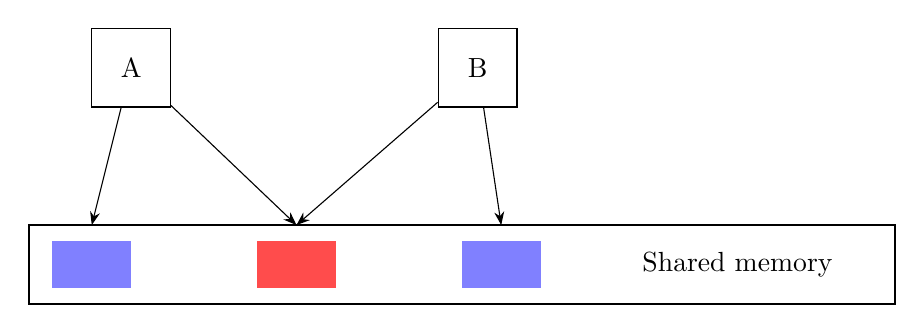
\begin{tikzpicture}[node distance=1cm and 1.5cm, >=Stealth]

        % Shared memory bar
        \draw[thick] (0,0) rectangle (11,1);
        \node at (9,0.5) {Shared memory};
      
        % Memory blocks
        \fill[blue!50] (0.3,0.2) rectangle (1.3,0.8);
        \fill[red!70] (2.9,0.2) rectangle (3.9,0.8);
        \fill[blue!50] (5.5,0.2) rectangle (6.5,0.8);
      
        % Processes A and B
        \node[draw, minimum width=1cm, minimum height=1cm] (A) at (1.3,3) {A};
        \node[draw, minimum width=1cm, minimum height=1cm] (B) at (5.7,3) {B};
      
        % Arrows from processes to memory blocks
        \draw[->] (A) -- (0.8,1);
        \draw[->] (A) -- (3.4,1);
        \draw[->] (B) -- (3.4,1);
        \draw[->] (B) -- (6.0,1);
      
      \end{tikzpicture}
      \caption{
        Shared-memory concurrency model. 
        Processes A and B communicate by reading and writing to shared memory blocks.
      }
      \label{fig:shared_memory}
\end{figure}

Note that the definition of \textit{memory} can be loosened depending on the application.
For example,~\cite{mitConcurrency} illustrates the following scenarios
where shared-memory concurrency models are applicable:

\begin{enumerate}
    \item A, B can be two processes communicating using the same process memory.
    \item A, B can be two programs communicating using the same filesystem.
    \item \label{itm:shared_object} A, B can be two running threads of some computer program
        communicating using the same object.
\end{enumerate}

When discussing limitations, advantages, or disadvantages of shared-memory concurrency models,
we will illustrate them using the scenario described in \autoref{itm:shared_object}.

\subsection{The Canonical Example}

The paper in~\cite{jaffe2011impactOfMemoryModels} describes a well-known canonical example.
Assume that we need to update a variable $x$ and increment it by $2$.
Assuming $x$ is already initialized, we can create two threads, $T_1$ and $T_2$, that will
increment $x$ by $1$ each. The code for both threads is shown in \autoref{fig:lost_update}.

Note that if both threads read the value of $x$ at the same time,
the final value of $x$ will be $1$. In fact, there's no guaranteed execution
order between $T_1$, and $T_2$ as the instructions can be interleaved
in any order. The interleaving problem is made more complex
due to the fact that most modern hardware can re-order instructions
\cite{huang2016debuggingConcurrentPrograms}. Furthermore, interleaving
makes it difficult to reproduce bugs, creating \textit{Heisenbugs}~\cite{rookout2021heisenbug,
gray1986whyComputersStop}.

\subsection{Problems with Shared-Memory Models}


%figure for the canonical example
\begin{figure}[!htp]
    \centering
    \begin{tabular}{|p{0.3\linewidth}|p{0.3\linewidth}|}
        \hline
        \textbf{$T_1$} & \textbf{$T_2$} \\
        \hline
        \begin{Verbatim}[fontsize=\small]
    int loc = x;
    loc = loc + 1;
    x = loc;
        \end{Verbatim}
        &
        \begin{Verbatim}[fontsize=\small]
    int loc = x;
    loc = loc + 1;
    x = loc;
        \end{Verbatim}
        \\
        \hline
    \end{tabular}
    \caption{Canonical example for shared-memory models.}
    \label{fig:lost_update}
\end{figure}

\section{Actor Model\label{sec:actor}}
An actor model is a type of concurrency model where the individual workers are the actors. An actor is an independent worker which has its own private state. Actors communicate by sending and receiving asynchronous messages. Each actor processes exactly one message at a time.

\subsection{Understanding the Actor Model Design}
The authors in~\cite{8316391} discuss the actor model design by first introducing the actor context. The actor context is the environment where the actors live. It creates actors, tracks them, routes messages to the right actor's mailbox.  The actor is the main unit of work done, in which each actor has a private state, has a mailbox attached, can send messages to other actors and process messages. The mailbox is where the incoming messages for the actor are stored. Processing is not done immediately, but whenever ready, the actor picks up a message from its mailbox and processes it. 
The actor model is illustrated in Figure~\ref{fig:actor}. 
\begin{figure}[H]
    \centering
    \includegraphics[width=0.7\textwidth]{actor.png}
    \caption{Actors communicating with other actors.}
    \label{fig:actor}
\end{figure}
\subsection{The Actor Model Principle}
The authors in~\cite{8316391} have also discussed regarding certain principles implemented in the actor model. Please refer to Table~\ref{tab:actor_model} for understanding the principles outlined in the actor model.

\begin{table}[H]
    \centering
    \caption{Basic Components of the Actor Model}
    \label{tab:actor_model}
    \begin{tabularx}{\textwidth}{|l|X|}
        \hline
        \textbf{Principle} & \textbf{Description} \\
        \hline
        Encapsulation & Each actor has a private internal state, and no actor can view it \\
        \hline
        Internal State & Each actor has its own memory and updates it. \\
        \hline
        Messaging & Actors communicate by sending and receiving \\
        \hline
        Indeterminacy & Messages may arrive in any order \\
        \hline
        
    \end{tabularx}
\end{table}

\subsection{Data Races and Deadlocks}
A data race occurs when when two or more threads access the same shared memory at the same time, which can corrupt the data. A deadlock occurs when two or more threads are waiting for each other to release a lock and so the system freezes. 

Data races don't occur in the actor model because there is no shared memory between actors, as each actor has its own private state, wherein no other actor can directly read or write that state and every communication happens through messages only. 

Deadlocks don't occur in the actor model as there is asynchronous messaging without any locks. Actors send a message and move on without waiting or blocking. In this no actor is waiting or holding a lock to release a resource.

\subsection{Optimization using Batch Actors}
The authors in~\cite{10820772} introduced batch actors to tackle the problem where hundreds of thousands of small tasks all try to synchronize through one actor, which can lead to a communication bottleneck.

Instead of using one main actor executing thousands of tasks, several tasks are grouped under batch actors, and batch actors message the main job actor, which leads to a reduce in contention. 

The experiments had shown that the models were 4x faster than the actor model without batching and resulted in less communication bottlenecks and better scaling.

\subsection{Benchmarks conducted}
The authors in~\cite{8892329} conducted various experiments using different libraries implementing the actor model. These were the findings:

\begin{table}[!htb]
    \centering
    \caption{Benchmarks and key findings from actor system implementations.}
    \label{tab:benchmarks_conducted}
    \begin{tabularx}{\textwidth}{|>{\raggedright\arraybackslash}X|>{\raggedright\arraybackslash}X|>{\raggedright\arraybackslash}X|}
        \hline
        \textbf{Benchmark} & \textbf{What it Measured} & \textbf{Main Finding} \\
        \hline
        Enqueuing Benchmark & Time taken to push messages into an actor's mailbox. & Scalaz achieved the fastest enqueuing time compared to Akka and Lift. \\
        \hline
        Max Throughput Benchmark & Number of messages processed per second. & Scalaz had the highest throughput performance. \\
        \hline
        Ping Latency Benchmark & Time for a message to travel from one actor to another and back. & Scalaz demonstrated the lowest ping latency. \\
        \hline
        Big Benchmark (Many-to-Many) & Performance under massive actor communication between many actors. & Scalaz scaled better with many actors under stress. \\
        \hline
        Chameneos Benchmark & Handling complex meeting and communication scenarios among actors. & Scalaz outperformed Akka and Lift in this concurrency problem. \\
        \hline
    \end{tabularx}
\end{table}

For pure speed, Scalaz is best for lightweight, fast concurrent systems. But for building robust, distributed systems, Akka is better because it offers more built-in tools as well as a good actor lifecycle management and for building complex and fault tolerant systems









\section{Software Transaction Memory\label{sec:stm}}
STM here

% Bibliography
\bibliographystyle{plain}
\bibliography{references}

\end{document}